\section{Multilagen-PVD}
\label{multilayer}

\todoline{LAMMPS und Parsivald von einander abheben: Parsivald nutzt auch LAMMPS, LAMMPS steht nachfolgend für reine MD-Simulationen}

Mit PVD-Methoden können auch mehrlagige Schichten abgeschieden werden, wie sie für röntgenoptische oder magnetische Systeme (Riesenmagnetowiderstand GMR, Tunnelmagnetowiderstand) interessant sind.
Im folgenden Abschnitt soll am Beispiel von dünnen \ce{Cu-Ni}-Multilagen ein System näher untersucht werden, welches zwar einen GMR-Effekt zeigt, aber in der Praxis von \ce{Cu-Co}-Systemen aufgrund des stärkeren GMR-Effektes abgelöst wurde\cite{bird_giant_1995}.
Das Kupfer-Nickel-System wurde aufgrund ähnlicher Gitterkonstanten gewählt (\ce{Ni}:~\SI{3.52}{\angstrom}, \ce{Cu}:~\SI{3.61}{\angstrom}), die epitaktisches Wachstum ermöglichen und somit Fehlstellen unterbinden.
Durch die Ähnlichkeit zur Kupfer-PVD lässt sich der Prozess zudem auf den dort entwickelten Prozessparametern und den untersuchten Potentialparametersätzen aufbauen.

Im Experiment werden mehrlagige Kupfer-Nickel-Schichten per Elektro\-deposition\cite{yang_pulsed_1995} oder durch Sputtern\cite{cammarata_nanoindentation_1990} hergestellt, wobei üblicherweise Lagendicken im Bereich mehrerer Nanometer erzielt werden.
Dieses Vorgehen lässt sich direkt in Parsivald-Simulationen übertragen, in denen zugunsten der Rechenzeit in den folgenden Untersuchungen vergleichsweise dünne Lagen mit einer Dicke von \SI{1}{\nano\meter} abgeschieden wurden.
Anschließend werden diese auf Ähnlichkeit mit LAMMPS-präparierten Multilagen hinsichtlich ihrer Lagendicke und -rauheit untersucht.
Eine Auswertung der relativen Verteilung der Spezies entlang der Abscheidungsrichtung wird ergänzend für verschiedene Relaxationszeiten als Maß der Lagenqualität durchgeführt.
Abscheidungen von Lagen mit einer Dicke von \SI{6}{\nano\meter} wurden ebenfalls mit Parsivald simuliert, doch mangels verfügbarer Rechenzeit für vergleichbare reine LAMMPS-Simulationen nicht eingehender untersucht.

Wie bei den Gold-PVD-Simulation zuvor müssen für erfolgreiche Simulationen einige Simulationsparameter wie Relaxationszeit, Thermostatdämpfung und Substrattemperatur optimiert werden.
Als Zielgrößen für die Optimierung wurden zur Vermeidung von Fehlstellen die Rauheit der Oberfläche und die Qualität der einzelnen Lagen im Vergleich mit ähnlichen Untersuchungen\cite{zhou_atomistic_1998} gewählt.
In diesen Untersuchungen wurde bereits gezeigt, dass die kinetische Energie der einfallenden Atome einen erheblichen Einfluss auf die Qualität der einzelnen Lagen hat, weshalb gleichartige Untersuchungen nur hinsichtlich der Substrattemperatur durchgeführt wurden.

\subsection{Ergebnisse}

Parsivald-Simulationen erzeugen nach korrekter Parametereinstellung klar abgegrenzte epitaktische Atomlagen geringer Rauheit, die sich gut mit den Ergebnissen gleichartiger LAMMPS-Simulationen decken (Abbildung~\ref{fig:multilayerresults}).
RMS-Rauheiten um \SI{1.2}{\angstrom} stellen sich mit beiden Simulationsmethoden bis zur zehnten Lage ein und stimmen somit untereinander und mit den bisherigen Ergebnissen überein (Abbildung~\ref{fig:multilayerplots-a}).
Anhand der Schichten ist eine schwach korrelierte Rauheit der einzelnen Lagen erkennbar.

Zuvor war eine Anpassung der Temperaturen und Relaxationszeiten notwendig, die jedoch für LAMMPS und Parsivald gleichermaßen gelten.
Als Richtwert wurde die Qualität der einzelnen Lagen in Form des Anteils der Spezies in Abhängigkeit der Höhe über dem Substrat genutzt (Abbildung~\ref{fig:multilayerplots-b}).
Lagen schlechterer Qualität zeigen eine höhere Durchmischung der Schichten\todo{Joerg: was aber auch korrekt sein kann, je nach Mischbarkeit}, was wiederum zu einer Senkung der relativen Häufigkeit einer Spezies innerhalb ihrer Schicht führt, wie für die beiden Verteilungen bei einer Relaxationszeit von \SI{0.2}{\femto\second} pro Ereignis beobachtet werden kann.
Erst bei Verdopplung der Relaxationszeit bilden sich \todo{Joerg: hier sollte man vielleicht irgendwo mal erwähnen, dass man das für dieses System erwartet? Eigentlich müsste man da was zu Mischbarkeit und Phasendiagramm der Legierungsbildung sagen ...}klar abgegrenzte Lagen aus, wie sie in Abbildung~\ref{fig:multilayerresults} dargestellt sind.

In Anhang~\ref{appendix:multilayer} ist eine Auswahl von mehrlagigen Kupfer-Nickel-Schichten dargestellt, die durch Unterrelaxation verursachte strukturelle Fehler aufweisen.
Bei größeren Systemen ist zudem mit dem Auftreten von Verspannungen aufgrund der leicht unterschiedlichen Bindungslängen sowie mit der Entstehung von Gitterversetzungen und Fehlstellen zu rechnen, die allerdings durch Finite-Size-Effekte unterdrückt sein können.

\begin{figure}
  \captionsetup[subfigure]{singlelinecheck=false}
  \def\subfigwidth{7cm}
  \begin{subfigure}[t]{\subfigwidth}
    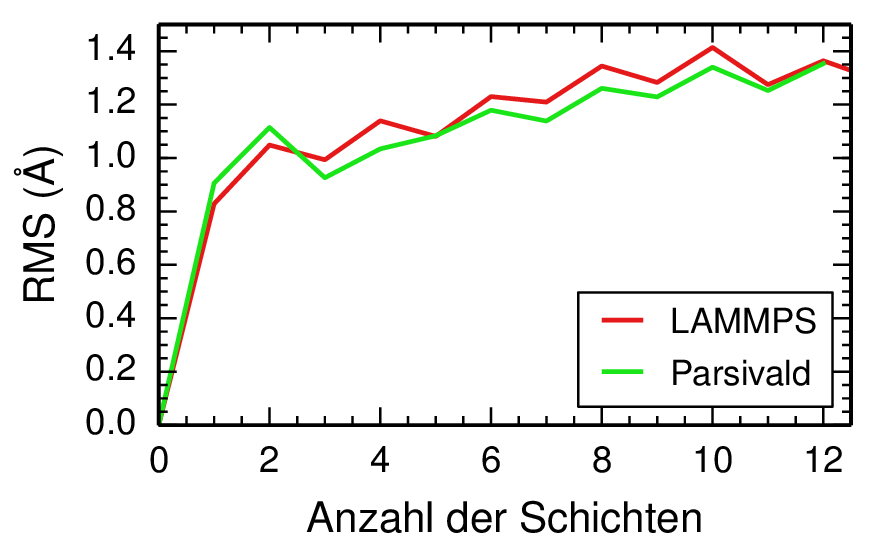
\includegraphics[width=\textwidth]{CuNi_layerroughness_comparison}
    \subcaption{
      Vergleich der Lagen-Rauheit (Abb.~\ref{fig:multilayerresults})
    }
    \label{fig:multilayerplots-a}
  \end{subfigure}
  \hfill
  \begin{subfigure}[t]{\subfigwidth}
    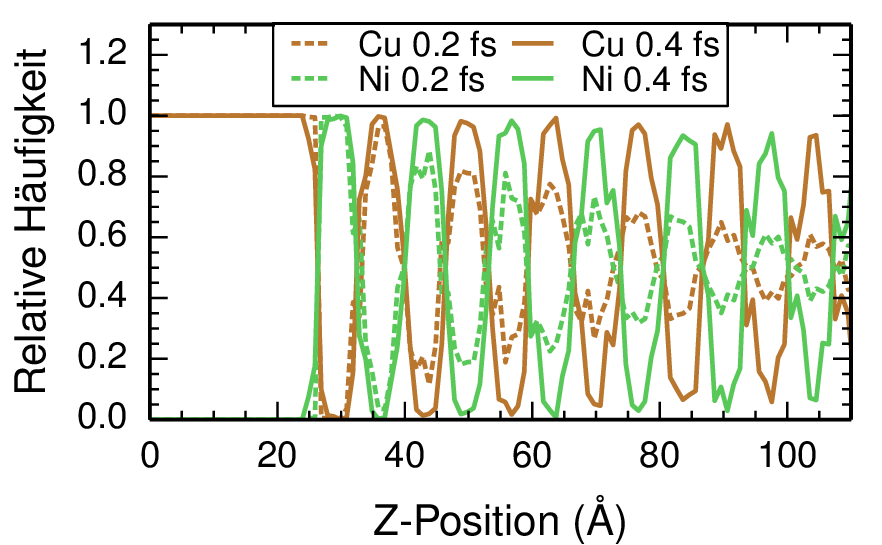
\includegraphics[width=\textwidth]{CuNi_atomdistribution_relax}
    \subcaption{Einfluss von $t_\text{relax}$ auf die Lagen-Qualität}
    \label{fig:multilayerplots-b}
  \end{subfigure}
  \caption[Rauheit und Qualität von Kupfer-Nickel-Multilagen]{
    Rauheit und Qualität von Kupfer-Nickel-Multilagen
  }
  \label{fig:multilayerplots}
\todoline{Joerg: etwas mehr Luft zwischen Kurven und Legende wäre hübsch}
\end{figure}

\begin{figure}
  \captionsetup[subfigure]{singlelinecheck=false}
  \def\subfigwidth{7cm}
  \begin{subfigure}[t]{\subfigwidth}
    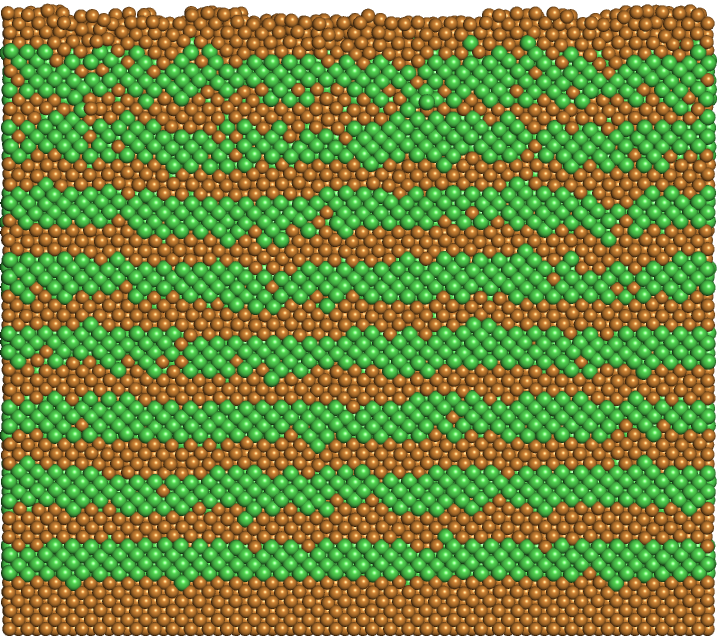
\includegraphics[width=\textwidth]{CuNi_profile_LAMMPS_nice}
    \subcaption{Profil von \ce{Cu-Ni}-Multilagen, reine MD-Simulation mit LAMMPS}
  \end{subfigure}
  \hfill
  \begin{subfigure}[t]{\subfigwidth}
    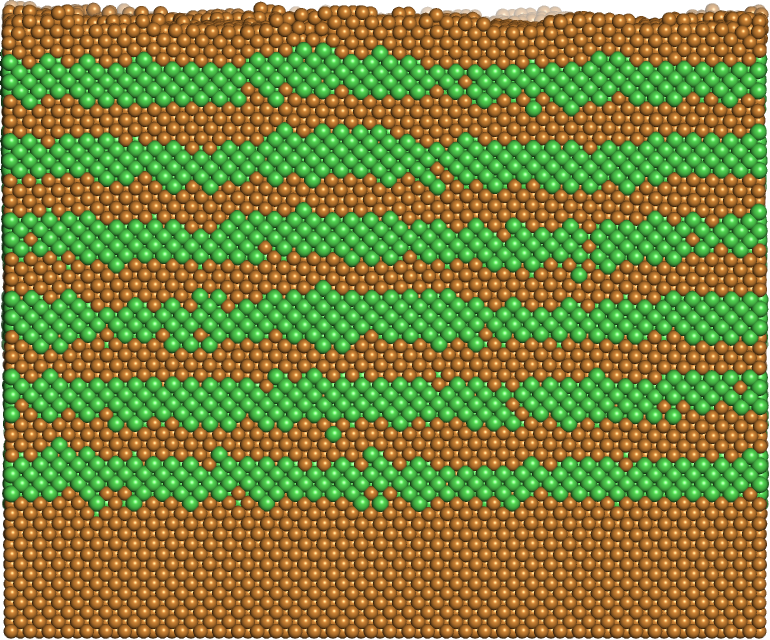
\includegraphics[width=\textwidth]{CuNi_profile_Parsivald}
    \subcaption{Profil von \ce{Cu-Ni}-Multilagen mit Parsivald}
  \end{subfigure}
  \caption{Vergleich von Multilagen-Profilen mit LAMMPS und Parsivald}
  \label{fig:multilayerresults}
\todoline{Joerg: Es wäre sinnvoll gewesen, identische Systeme zu rechnen ...}
\end{figure}

\todoline{Joerg: Fazit der schönen Ergebnisse (Übereinstimmung LAMMPS und Parsivald)}
\todoline{Laufzeiten usw. schnell vergleichen}
